\apendice{Especificación de Requisitos}

\section{Introducción}

Esta sección explicará los requerimientos funcionales, no funcionales y casos de uso de la aplicación desarrollada.

\section{Objetivos generales}

El objetivo principal de este proyecto es desarrollar una herramienta web docente orientada a facilitar la enseñanza y el aprendizaje del algoritmo de árboles de decisión C4.5. La aplicación pretende ofrecer una explicación interactiva de los conceptos teóricos necesarios para comprender el funcionamiento del algoritmo, así como una simulación visual y paso a paso de la construcción y la poda de un árbol de decisión.

La herramienta se estructura en tres apartados principales. El primero está dedicado al cálculo de la entropía y de la entropía condicional. En estas secciones, el usuario puede introducir valores personalizados, añadir o eliminar clases o categorías y consultar los resultados obtenidos. Además, en el caso de trabajar con dos clases, la aplicación permite representar visualmente el resultado del cálculo de entropía mediante una gráfica de entropía binaria.

El segundo apartado corresponde a la elección de nodo. Esta sección permite estudiar de manera detallada los cálculos realizados por el algoritmo C4.5 durante cada iteración. El usuario puede consultar las fórmulas asociadas a cada concepto, sustituir los valores de los parámetros y comprobar el resultado de los cálculos. Asimismo, puede generar de forma automática una tabla de datos personalizada y analizar los valores obtenidos para el cálculo de umbrales, la ganancia de información, el \textit{split info} y el \textit{gain ratio} .

Además, esta sección incorpora mecanismos de navegación contextual que permiten acceder a la explicación de un cálculo concreto desde las tablas de resultados. De esta forma, el usuario puede comprender el origen de los valores mostrados sin necesidad de introducir de nuevo los datos utilizados. También se muestra gráficamente el nodo seleccionado por el algoritmo, junto con una leyenda explicativa que facilita la interpretación de las condiciones de las ramas y de las hojas generadas.

El tercer apartado corresponde a la simulación del algoritmo C4.5. En esta sección, el usuario puede utilizar conjuntos de datos de ejemplo o cargar un archivo CSV propio para generar un árbol de decisión. La simulación se divide en dos partes diferenciadas: la construcción paso a paso del árbol y el proceso de poda. Ambas permiten avanzar y retroceder entre las distintas iteraciones, consultar los cálculos asociados y observar los cambios producidos en la estructura del árbol.

La aplicación incorpora también diferentes mecanismos de visualización para facilitar la comprensión de árboles de gran tamaño. Entre ellos se incluyen paneles retráctiles, herramientas de ampliación, una lupa para observar zonas concretas del árbol y un sistema de seguimiento del último nodo o hoja generado. Estas funcionalidades permiten mejorar la legibilidad de la representación y adaptar la interfaz a las necesidades del usuario durante la simulación.

\section{Catálogo de requisitos}

\subsection{Requisitos funcionales}

\begin{itemize}
\item \textbf{FR-1} Desde la aplicación web, el usuario debe poder calcular la entropía y la entropía condicional a partir de los valores que introduzca.

\begin{itemize}
    \item \textbf{FR-1.1} El usuario debe poder introducir valores numéricos correspondientes al número de instancias de cada clase para calcular la entropía.

    \item \textbf{FR-1.2} El usuario debe poder añadir nuevas clases mediante el botón habilitado para ello.

    \item \textbf{FR-1.3} El usuario debe poder eliminar la última clase añadida.

    \item \textbf{FR-1.4} El usuario debe poder iniciar el cálculo de la entropía mediante el botón correspondiente.

    \item \textbf{FR-1.5} La aplicación debe calcular correctamente la probabilidad asociada a cada clase y el valor total de la entropía.

    \item \textbf{FR-1.6} Cuando el usuario utilice dos clases, la aplicación debe mostrar la representación del resultado en la gráfica de entropía binaria.

    \item \textbf{FR-1.7} El usuario debe poder introducir valores correspondientes a las diferentes categorías y clases para calcular la entropía condicional.

    \item \textbf{FR-1.8} El usuario debe poder añadir nuevas categorías y eliminar la última categoría añadida.

    \item \textbf{FR-1.9} El usuario debe poder iniciar el cálculo de la entropía condicional mediante el botón correspondiente.

    \item \textbf{FR-1.10} La aplicación debe calcular correctamente la proporción de cada categoría, su entropía y el valor total de la entropía condicional.
\end{itemize}

\item \textbf{FR-2} Desde la aplicación web, el usuario debe poder calcular los distintos elementos que intervienen en la elección de nodo del algoritmo C4.5 a partir de valores definidos por él mismo.

\begin{itemize}
    \item \textbf{FR-2.1} El usuario debe poder introducir valores en las celdas disponibles para sustituir los parámetros mostrados en las fórmulas de cada cálculo.

    \item \textbf{FR-2.2} El usuario debe poder pulsar el botón de cálculo para obtener el resultado correspondiente a los valores introducidos.

    \item \textbf{FR-2.3} La aplicación debe calcular los resultados utilizando las fórmulas mostradas en pantalla.

    \item \textbf{FR-2.4} El usuario debe poder configurar los valores mínimo y máximo utilizados para generar los datos, las variables de clase y el número de filas de una tabla dinámica.

    \item \textbf{FR-2.5} El usuario debe poder generar una tabla de datos aleatoria a partir de los parámetros introducidos previamente.

    \item \textbf{FR-2.6} El usuario debe poder calcular los umbrales candidatos de los atributos numéricos mediante el botón correspondiente.

    \item \textbf{FR-2.7} La aplicación debe mostrar los datos ordenados y los valores calculados necesarios para analizar los umbrales candidatos.

    \item \textbf{FR-2.8} La aplicación debe calcular y mostrar la ganancia de información, el \textit{split info} y el \textit{gain ratio}  de los atributos evaluados.

    \item \textbf{FR-2.9} El usuario debe poder seleccionar determinadas celdas de las tablas de resultados para acceder a la sección en la que se explica el cálculo asociado a ese valor.

    \item \textbf{FR-2.10} La aplicación debe conservar los datos utilizados por el usuario al navegar entre las secciones relacionadas.

    \item \textbf{FR-2.11} El usuario debe poder visualizar leyendas explicativas que faciliten la comprensión de los elementos presentes en las tablas de datos ordenados y de valores calculados.

    \item \textbf{FR-2.12} En el apartado de elección de nodo, la aplicación debe mostrar mediante una representación gráfica el nodo seleccionado a partir de la tabla generada.

    \item \textbf{FR-2.13} La aplicación debe mostrar una leyenda bajo la representación gráfica del nodo elegido, explicando aspectos como el significado de las hojas definitivas y las condiciones asociadas a las ramas.
\end{itemize}

\item \textbf{FR-3} Desde la aplicación web, el usuario debe poder acceder a la simulación paso a paso de la construcción y la poda de un árbol de decisión mediante el algoritmo C4.5.

\begin{itemize}
    \item \textbf{FR-3.1} El usuario debe poder seleccionar uno de los conjuntos de datos de ejemplo disponibles para ejecutar la simulación.

    \item \textbf{FR-3.2} El usuario debe poder cargar un archivo CSV propio mediante el botón de subida de archivos.

    \item \textbf{FR-3.3} El usuario debe poder seleccionar el criterio de elección de nodos entre ganancia de información y \textit{gain ratio}.

    \item \textbf{FR-3.4} El usuario debe poder eliminar el conjunto de datos cargado y reiniciar la simulación mediante el botón de limpieza.

    \item \textbf{FR-3.5} El usuario debe poder contraer y expandir los paneles correspondientes al árbol, al conjunto de datos y a los cálculos para adaptar la visualización a sus necesidades.

    \item \textbf{FR-3.6} El usuario debe poder aumentar y reducir el nivel de ampliación del árbol mediante los botones habilitados para ello.

    \item \textbf{FR-3.7} El usuario debe poder utilizar una herramienta de lupa para observar con mayor detalle una zona concreta del árbol sobre la que sitúe el cursor.

    \item \textbf{FR-3.8} El usuario debe poder acceder directamente a la última iteración de la simulación mediante el botón correspondiente.

    \item \textbf{FR-3.9} El usuario debe poder regresar directamente a la primera iteración de la simulación mediante el botón correspondiente.

    \item \textbf{FR-3.10} El usuario debe poder avanzar o retroceder una iteración mediante los botones de navegación de pasos.

    \item \textbf{FR-3.11} Cuando el usuario seleccione un conjunto de datos de ejemplo, debe poder consultar la fuente o una explicación relacionada con dicho conjunto de datos.

    \item \textbf{FR-3.12} El usuario debe poder navegar entre las pestañas de simulación de construcción del árbol C4.5 y de simulación de poda.

    \item \textbf{FR-3.13} Durante la construcción del árbol, la aplicación debe mostrar el conjunto de datos, los cálculos realizados y la estructura del árbol correspondiente al paso actual.

    \item \textbf{FR-3.14} Durante la simulación de poda, la aplicación debe mostrar el nodo o subárbol evaluado, los cálculos asociados y la decisión final sobre si el subárbol se mantiene o se sustituye por una hoja.

    \item \textbf{FR-3.15} La aplicación debe resaltar y centrar automáticamente el último nodo o hoja generado durante cada paso de la simulación.

    \item \textbf{FR-3.16} Cuando el usuario seleccione la ganancia de información como criterio de elección, la aplicación debe informar de que el \textit{gain ratio}  es el criterio de decisión propio del algoritmo C4.5.
\end{itemize}


\end{itemize}

\subsection{Requisitos no funcionales}

\begin{itemize}
\item \textbf{NFR-1} La interfaz de usuario debe ser sencilla, intuitiva y adecuada para usuarios que no dispongan de conocimientos previos sobre el algoritmo C4.5.


\item \textbf{NFR-2} La aplicación debe adaptarse a diferentes tamaños y resoluciones de pantalla, manteniendo la legibilidad de sus elementos principales.

\item \textbf{NFR-3} La aplicación debe validar los archivos CSV antes de iniciar la simulación para evitar errores de procesamiento y de representación.

\begin{itemize}
    \item \textbf{NFR-3.1} El archivo debe estar en formato CSV y utilizar la coma como separador de valores.

    \item \textbf{NFR-3.2} La primera fila del archivo debe contener los nombres de los atributos o cabeceras de las columnas.

    \item \textbf{NFR-3.3} El conjunto de datos no debe contener más de 150 filas de datos.

    \item \textbf{NFR-3.4} El archivo no debe contener más de 25 columnas.

    \item \textbf{NFR-3.5} La cabecera no debe contener columnas vacías.

    \item \textbf{NFR-3.6} Todas las filas deben contener el mismo número de columnas.

    \item \textbf{NFR-3.7} No se permiten valores vacíos dentro del conjunto de datos.

    \item \textbf{NFR-3.8} Todos los valores de una misma columna deben pertenecer al mismo tipo de dato.

    \item \textbf{NFR-3.9} Los tipos de datos admitidos son numérico, booleano y categórico.

    \item \textbf{NFR-3.10} La última columna debe corresponder a la clase objetivo del conjunto de datos.

    \item \textbf{NFR-3.11} La columna de clase debe contener exactamente dos valores distintos.

    \item \textbf{NFR-3.12} La aplicación debe informar al usuario mediante un mensaje comprensible cuando el archivo CSV no cumpla alguno de los requisitos establecidos.
\end{itemize}

\item \textbf{NFR-5} La representación de árboles generados a partir de conjuntos de datos próximos a los límites admitidos debe mantenerse legible mediante las herramientas de ampliación, lupa, paneles retráctiles y ayudas contextuales disponibles.

\end{itemize}

\section{Catálogo de requisitos}

En la figura \ref{Fig_B.1} se muestra el diagrama de caso de uso del usuario de la aplicación.

\begin{figure}[htbp]
     \centering
     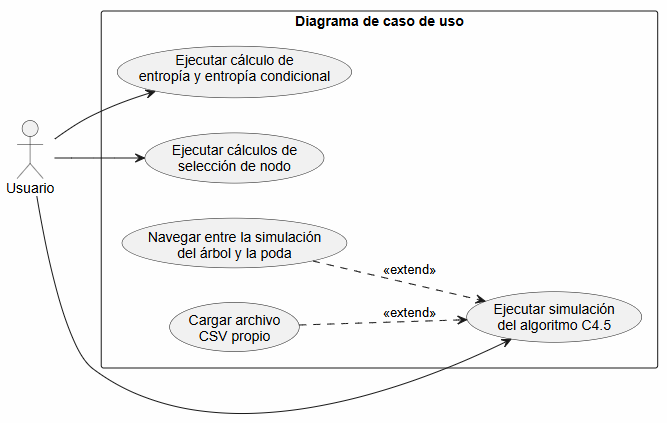
\includegraphics[width=0.75\textwidth]{img/Diagrama_Caso_uso.png}
     \caption{Diagrama de caso de uso de la aplicación}
     \label{Fig_B.1}
 \end{figure}
 
El diagrama describe al usuario de la aplicación web como el único actor y al Simulador del algoritmo C4.5 como el sistema que contiene todos los casos de uso dentro de sus límites. El usuario interactúa directamente con los tres casos de uso principales: ejecutar las calculadoras de entropía y entropía condicional, realizar los cálculos de elección de nodo y ejecutar la simulación del algoritmo C4.5.

Dentro de la simulación del algoritmo C4.5, el usuario puede cargar de forma opcional un conjunto de datos propio en formato CSV, como alternativa a los conjuntos de datos de ejemplo disponibles. Además, el usuario puede navegar entre la simulación de construcción del árbol C4.5 y la simulación del proceso de poda. Estas dos funcionalidades se representan como extensiones del caso de uso principal denominado ``Ejecutar simulación del algoritmo C4.5''.


\subsection{Casos de uso}

El sistema contiene cinco casos de uso. El caso de uso textual Ejecutar cálculos de entropía y entropía condicional'' se presenta en la Tabla \ref{tabla:uc_1}; el caso de uso Ejecutar cálculos de elección de nodo'' se muestra en la Tabla \ref{tabla:uc_2}; la tabla recoge el caso de uso denominado ``Ejecutar simulación del algoritmo C4.5''.

Asimismo, el caso de uso Cargar archivo CSV propio'', que actúa como una extensión de la simulación principal, se describe en la Tabla \ref{tabla:uc_4}. Finalmente, la Tabla \ref{tabla:uc_5} presenta el caso de uso Navegar entre la simulación del árbol y la poda'', también representado como una extensión de la simulación del algoritmo C4.5.

% Caso de uso 1
\begin{table}[p]
    \centering
    \begin{tabularx}{\linewidth}{p{0.21\columnwidth} p{0.71\columnwidth}}
        \toprule
        \textbf{UC-1} & \textbf{Ejecutar cálculos de entropía y entropía condicional} \\
        \toprule
        \textbf{Versión} & 1.0 \\
        \textbf{Autor} & Marcos Guzmán Asolas \\
        \textbf{Requisitos asociados} & FR-1, FR-1.1, FR-1.2, FR-1.3, FR-1.4, FR-1.5, FR-1.6, FR-1.7, FR-1.8, FR-1.9 y FR-1.10. \\
        \textbf{Descripción} & El usuario utiliza las calculadoras de entropía y entropía condicional para introducir valores personalizados y consultar los resultados generados por la aplicación. \\
        \textbf{Precondición} & El usuario ha accedido a la aplicación web. \\
        \textbf{Acciones} &
        \begin{enumerate}
            \def\labelenumi{\arabic{enumi}.}
            \tightlist
            \item El usuario accede a la sección de entropía o entropía condicional.
            \item El usuario introduce los valores requeridos en los campos disponibles.
            \begin{enumerate}
                \item En el cálculo de entropía, el usuario puede añadir o eliminar clases.
                \item En el cálculo de entropía condicional, el usuario puede añadir o eliminar categorías.
            \end{enumerate}
            \item El usuario pulsa el botón correspondiente para iniciar el cálculo.
            \item La aplicación valida los valores introducidos.
            \item La aplicación calcula y muestra los resultados.
            \begin{enumerate}
                \item En el cálculo de entropía, se muestran las probabilidades de cada clase y el valor total de la entropía.
                \item Si se utilizan dos clases, la aplicación representa el resultado en la gráfica de entropía binaria.
                \item En el cálculo de entropía condicional, se muestran la proporción, la entropía de cada categoría y el valor final de la entropía condicional.
            \end{enumerate}
        \end{enumerate} \\
        \textbf{Postcondición} & Los resultados del cálculo solicitado se muestran en la tabla correspondiente. \\
        \textbf{Excepciones} & Si el usuario introduce valores no válidos, la aplicación muestra un aviso indicando que deben introducirse valores numéricos positivos. \\
        \textbf{Importancia} & Alta \\
        \bottomrule
    \end{tabularx}
    \caption{UC-1 Ejecutar cálculos de entropía y entropía condicional.}
    \label{tabla:uc_1}
\end{table}


% Caso de uso 2
\begin{table}[p]
    \centering
    \begin{tabularx}{\linewidth}{p{0.21\columnwidth} p{0.71\columnwidth}}
        \toprule
        \textbf{UC-2} & \textbf{Ejecutar cálculos de elección de nodo} \\
        \toprule
        \textbf{Versión} & 1.0 \\
        \textbf{Autor} & Marcos Guzmán Asolas \\
        \textbf{Requisitos asociados} & FR-2, FR-2.1, FR-2.2, FR-2.3, FR-2.4, FR-2.5, FR-2.6, FR-2.7, FR-2.8, FR-2.9, FR-2.10, FR-2.11, FR-2.12 y FR-2.13. \\
        \textbf{Descripción} & El usuario consulta y realiza los cálculos necesarios para comprender el proceso de elección de nodo del algoritmo C4.5, incluyendo el cálculo de umbrales, ganancia de información, información de división y razón de ganancia. \\
        \textbf{Precondición} & El usuario ha accedido a la sección de elección de nodo. \\
        \textbf{Acciones} &
        \begin{enumerate}
            \def\labelenumi{\arabic{enumi}.}
            \tightlist
            \item El usuario selecciona uno de los apartados de cálculo disponibles.
            \item El usuario puede introducir valores manualmente en las celdas asociadas a la fórmula mostrada.
            \item El usuario pulsa el botón de cálculo.
            \item La aplicación calcula y muestra el resultado de acuerdo con la fórmula correspondiente.
            \item De forma alternativa, el usuario configura los parámetros necesarios para generar una tabla dinámica.
            \item El usuario pulsa el botón de generación de tabla.
            \item La aplicación genera una tabla de datos aleatoria a partir de los parámetros establecidos.
            \item El usuario pulsa el botón para calcular los umbrales candidatos.
            \item La aplicación muestra los datos ordenados y los valores calculados correspondientes.
            \item El usuario puede seleccionar una celda de las tablas de resultados para acceder a la explicación del cálculo asociado.
            \item La aplicación muestra el nodo seleccionado y una leyenda explicativa sobre las condiciones de las ramas y las hojas generadas.
        \end{enumerate} \\
        \textbf{Postcondición} & El usuario visualiza los cálculos realizados y si el usuario se encuentra en el subapartado de nodo elegido, se visualiza la representación del nodo seleccionado para el conjunto de datos utilizado. \\
        \textbf{Excepciones} & Si los valores introducidos no son válidos o no permiten realizar el cálculo, la aplicación muestra un mensaje informativo al usuario. \\
        \textbf{Importancia} & Alta \\
        \bottomrule
    \end{tabularx}
    \caption{UC-2 Ejecutar cálculos de elección de nodo.}
    \label{tabla:uc_2}
\end{table}


% Caso de uso 3
\begin{table}[p]
    \centering
    \begin{tabularx}{\linewidth}{p{0.21\columnwidth} p{0.71\columnwidth}}
        \toprule
        \textbf{UC-3} & \textbf{Ejecutar simulación del algoritmo C4.5} \\
        \toprule
        \textbf{Versión} & 1.0 \\
        \textbf{Autor} & Marcos Guzmán Asolas \\
        \textbf{Requisitos asociados} & FR-3, FR-3.1, FR-3.3, FR-3.4, FR-3.5, FR-3.6, FR-3.7, FR-3.8, FR-3.9, FR-3.10, FR-3.11, FR-3.13, FR-3.14 y FR-3.15. \\
        \textbf{Descripción} & El usuario ejecuta una simulación paso a paso del algoritmo C4.5 utilizando un conjunto de datos de ejemplo y consulta la construcción progresiva del árbol, los cálculos realizados y la estructura generada. \\
        \textbf{Precondición} & El usuario ha accedido a la sección de simulación del algoritmo C4.5. \\
        \textbf{Acciones} &
        \begin{enumerate}
            \def\labelenumi{\arabic{enumi}.}
            \tightlist
            \item El usuario selecciona uno de los conjuntos de datos de ejemplo disponibles.
            \item La aplicación carga el conjunto de datos seleccionado.
            \item El usuario selecciona el criterio de visualización de la elección de nodo.
            \item La aplicación genera la simulación correspondiente al conjunto de datos y al criterio seleccionado.
            \item La aplicación muestra el árbol de decisión, el conjunto de datos y los cálculos asociados al paso actual.
            \item El usuario navega por la simulación mediante los botones de navegación.
            \item El usuario puede contraer o expandir los paneles disponibles.
            \item El usuario puede aumentar o reducir el nivel de ampliación del árbol.
            \item El usuario puede utilizar la herramienta de lupa para observar una zona concreta del árbol.
            \item La aplicación centra y resalta el último nodo o hoja generado en cada paso.
            \item El usuario puede consultar la fuente o la explicación del conjunto de datos de ejemplo seleccionado.
        \end{enumerate} \\
        \textbf{Postcondición} & El árbol de decisión, los datos y los cálculos se muestran en la iteración seleccionada por el usuario. \\
        \textbf{Excepciones} & Si el usuario selecciona la ganancia de información como criterio de visualización, la aplicación muestra un aviso indicando que el criterio propio del algoritmo C4.5 es la razón de ganancia. \\
        \textbf{Importancia} & Alta \\
        \bottomrule
    \end{tabularx}
    \caption{UC-3 Ejecutar simulación del algoritmo C4.5.}
    \label{tabla:uc_3}
\end{table}


% Caso de uso 4
\begin{table}[p]
    \centering
    \begin{tabularx}{\linewidth}{p{0.21\columnwidth} p{0.71\columnwidth}}
        \toprule
        \textbf{UC-4} & \textbf{Cargar archivo CSV propio} \\
        \toprule
        \textbf{Versión} & 1.0 \\
        \textbf{Autor} & Marcos Guzmán Asolas \\
        \textbf{Requisitos asociados} & FR-3.2, NFR-3, NFR-3.1, NFR-3.2, NFR-3.3, NFR-3.4, NFR-3.5, NFR-3.6, NFR-3.7, NFR-3.8, NFR-3.9, NFR-3.10, NFR-3.11 y NFR-3.12. \\
        \textbf{Descripción} & Dentro de la simulación del algoritmo C4.5, el usuario carga un conjunto de datos propio en formato CSV para generar y analizar el árbol de decisión resultante. \\
        \textbf{Precondición} & El usuario ha accedido a la sección de simulación del algoritmo C4.5. \\
        \textbf{Acciones} &
        \begin{enumerate}
            \def\labelenumi{\arabic{enumi}.}
            \tightlist
            \item El usuario pulsa el botón de carga de archivo CSV.
            \item La aplicación muestra una ventana modal con los requisitos que debe cumplir el archivo.
            \item El usuario selecciona un archivo CSV desde su dispositivo.
            \item La aplicación valida el archivo seleccionado.
            \begin{enumerate}
                \item La aplicación comprueba que el archivo utiliza la coma como separador.
                \item La aplicación comprueba que existe una cabecera sin columnas vacías.
                \item La aplicación comprueba que el archivo no supera las 150 filas ni las 25 columnas.
                \item La aplicación comprueba que todas las filas tienen el mismo número de columnas.
                \item La aplicación comprueba que no existen valores vacíos.
                \item La aplicación comprueba que los datos de cada columna son del mismo tipo.
                \item La aplicación comprueba que la última columna contiene la clase objetivo y dos valores distintos.
            \end{enumerate}
            \item Si el archivo es válido, la aplicación carga el conjunto de datos y genera la simulación.
        \end{enumerate} \\
        \textbf{Postcondición} & El conjunto de datos seleccionado por el usuario se carga y queda disponible para ejecutar la simulación del algoritmo C4.5. \\
        \textbf{Excepciones} & Si el archivo no cumple alguno de los requisitos definidos, la aplicación muestra un mensaje indicando el requisito incumplido y no carga el conjunto de datos. \\
        \textbf{Importancia} & Media \\
        \bottomrule
    \end{tabularx}
    \caption{UC-4 Cargar archivo CSV propio.}
    \label{tabla:uc_4}
\end{table}


% Caso de uso 5
\begin{table}[p]
    \centering
    \begin{tabularx}{\linewidth}{p{0.21\columnwidth} p{0.71\columnwidth}}
        \toprule
        \textbf{UC-5} & \textbf{Navegar entre la simulación del árbol y la poda} \\
        \toprule
        \textbf{Versión} & 1.0 \\
        \textbf{Autor} & Marcos Guzmán Asolas \\
        \textbf{Requisitos asociados} & FR-3.12, FR-3.13 y FR-3.14. \\
        \textbf{Descripción} & Dentro de la simulación del algoritmo C4.5, el usuario navega entre la simulación de construcción del árbol y la simulación del proceso de poda. \\
        \textbf{Precondición} & El usuario ha cargado un conjunto de datos válido y se encuentra en la sección de simulación del algoritmo C4.5. \\
        \textbf{Acciones} &
        \begin{enumerate}
            \def\labelenumi{\arabic{enumi}.}
            \tightlist
            \item El usuario accede a la sección de simulación del algoritmo C4.5.
            \item La aplicación muestra las pestañas correspondientes a la simulación de construcción del árbol y a la simulación de poda.
            \item El usuario selecciona la pestaña de simulación del árbol C4.5.
            \item La aplicación muestra los pasos de construcción del árbol, el conjunto de datos, los cálculos y la estructura generada.
            \item El usuario selecciona la pestaña de poda.
            \item La aplicación muestra el nodo o subárbol evaluado, los cálculos de poda y la decisión correspondiente.
            \item El usuario puede alternar entre ambas pestañas en cualquier momento.
        \end{enumerate} \\
        \textbf{Postcondición} & El usuario visualiza la simulación de construcción del árbol o la simulación de poda seleccionada. \\
        \textbf{Excepciones} & Si no se ha cargado un conjunto de datos válido, la aplicación no permite iniciar la simulación de construcción ni la simulación de poda. \\
        \textbf{Importancia} & Alta \\
        \bottomrule
    \end{tabularx}
    \caption{UC-5 Navegar entre la simulación del árbol y la poda.}
    \label{tabla:uc_5}
\end{table}


